\chapter{Summary and concluding remarks}\label{CH_summary}

\section{Conclusions}

In this thesis we investigated the evolution of galaxies by studying the growth of stellar mass and stellar mass density in time in the last 6 Gyr. We combined the datasets from two very large surveys and built the largest catalog of galaxies to date that has consistent fluxes in 5 optical (SDSS) and 2 near-IR (WISE) bands and contains over 9 million galaxies. This consistency has been achieved in two ways:\\ 
- in optical all bands were convolved with the PSF of the band with the worst FWHM, namely u-band. We did this by constructing PSF functions for each individual SDSS image. Then, using r\_matched\_u band as a detection image we extracted fluxes of the sources sources in SDSS Stripe 82 field.\\
- in near-IR the angular resolution is $\approx 6$ times worse than in optical, so we applied "template-fitting" technique in which we use the high-resolution image to define the morphological template of the galaxy in question, and de-convolve its light profile in the low-resolution image.

This approach allows us to perform SED measurements in the restframe near-IR regime, which is important for the correct estimation of the dust extinction and contribution of the low-mass stars, which may be outshone by brighter stars in optical, and thus are accountant, but contribute significantly to the total stellar mass of the galaxy. We derive photometric redshifts and stellar masses for all the 9 million galaxies that span at $z=0$-0.8 and calculated stellar mass density over four redshift bins. Our SMD (we call it low-limits, since we did not correct for incompleteness of low-mass galaxies in the higher redshift bins) are generally close to the previously reported results, but with a much larger statistics over significant portion of the sky. Our result contribute to the GSMD and shall be used in future to provide constraints on any models of the galaxy evolution at high redshifts.

\section{Future work}

In 2010, after the depletion of coolant in the WISE telescope, w3 and w4 became unusable. Nevertheless, WISE continued surveying the sky through January 2011 in w1 and w2 as they are less affected by the rising temperature of the sensor, including a portion of the mission referred to as NEOWISE \citep{2011ApJ...731...53M}. WISE was placed in hibernation in February 2011, and was later reactivated in October 2013 and continued surveying the sky in w1 and w2. This survey is referred to as NEOWISE-Reactivation (NEOWISER) and continued until 2017. NEOWISER images are of very nearly the same high quality as those of the pre-hibernation WISE mission and it was quickly appreciated by the astronomical community. \citep{1538-3881-154-4-161} created a set of co-add images following procedures in D14 for all available data in bands w1 and w2. This not only made the images more sensitive (by 0.38 magnitudes in both bands), but significantly reduce the noise and allowed to clean out transient and spurious sources. That is very important to us because as you may see in the Figure~\ref{fig:sm_w1-mag} lots (58\%) of the sources are below the detection limit. We still supply such sources to TPHOT for the reasons to be explained in the next subsection, but their near-IR magnitudes are untrustworthy. New data from \citep{1538-3881-154-4-161} will add 5\% more sources above the detection limit and make stellar mass estimation more robust.

\begin{figure}[!ht]
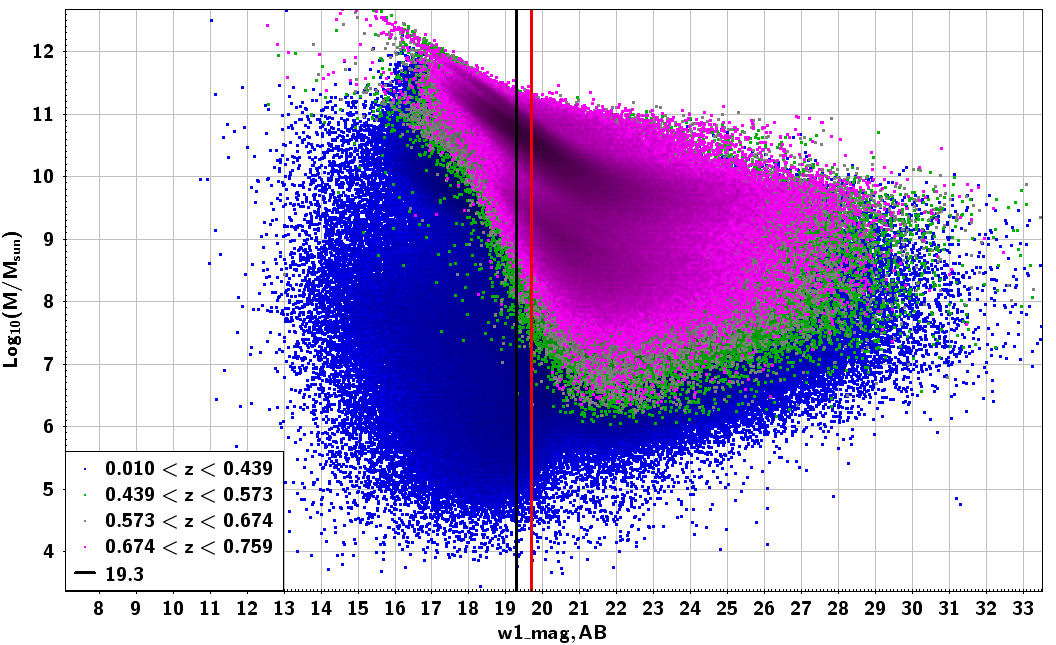
\includegraphics[width=6in]{Figures/mass_vs_w1-mag.png}
\caption{Stellar masses are plotted over corresponding w1-band magnitudes. Four redshift bins are plotted in different colors: z1 - blue, z2 - green, z3 - grey, z4 - magenta. Black vertical line denotes the $5\sigma$ detection limit for unWISE, red vertical image - analogous detection limit for the stacked WISE and NEOWISER data}
\label{fig:sm_w1-mag}
\end{figure}

In order to use these images we need to construct 240 new PSFs per band (480 in total) convolve them to already existing r\_matched\_u PSFs and re-run the TPHOT over entire Stripe 82 region. Such run, though time-consuming, will not only significantly increase the precision of the near-IR photometry, but also increase the total number of sources. In deeper near-IR images more sources will have non-zero fluxes - so sources that now have photometric fluxes in less then 4 bands and are currently not supplied for SED fitting will be included in the stellar mass density estimation. 

\subsection{Optical dropouts in WISE}
Residuals in w1 and w2 that are produced by TPHOT reveal a mysterious population of objects with SNR$>5$ in both bands. The fact that they were not "cleaned out" by TPHOT suggests that they are invisible in optical and our inspection of SDSS images proves this. We call them "WISE optical dropouts" (WoDrops) and investigating their nature is a follow-up for this project, though some preparatory work has been already done.\\
- Using the latter WISE observations in w1 and w2 during "3-Band Cryo" and "NEOWISE" programs, we verified that these objects cannot be transients.\\
- Their colors ($w1-z>4.8$ AB mag) cannot be explained by Galactic brown dwarfs.\\
- WoDrops cannot be a high-redshift ($z>7$) objects due to their large number density (\~176/square degree) - that contradicts to current observations of the population of the most luminous quasars.\\
An example of such WoDrop is presented in Figure~\ref{fig:wodrop_sdss}

\begin{figure}[!ht]
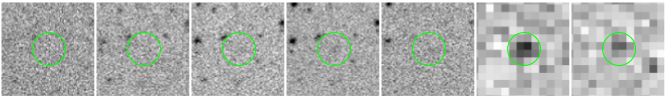
\includegraphics[width=6in]{Figures/wodrop_sdss_w1w2.png}
\caption{An example of WoDrop. Shown from left to right are the $ugriz$ and unWISE w1 and w2 images. The images are 33"x33" in size, and the green circles indicate the location of the WoDrop. For this particular example is SNR = 8 and 5.4 for bands w1 and w2 respectively.}
\label{fig:wodrop_sdss}
\end{figure}

The only reasonable explanation is that these objects may be a low-redshift (z$\sim0.5$) old, massive but passive galaxies that resemble in colors Spitzer IRAC-selected Extremely Red Objects (IERO) \citep{Yan2004}. If this is really the case then our low-$z$ stellar mass density may be underestimated. In order to better understand the nature of such objects we need data in the near-IR regime, namely filters J, H and Ks - they lie in between optical filters $ugriz$ and w1, w2 bands. Figure~\ref{fig:wodrop_sed} shows an example of the SED fitting for one of the WoDrops. w1 and w2 photometry is shown in magenta, non-detection in optical bands is plotted with upper-limits in grey and possible photometry for J, H and Ks bands is in blue.

\begin{figure}[!ht]
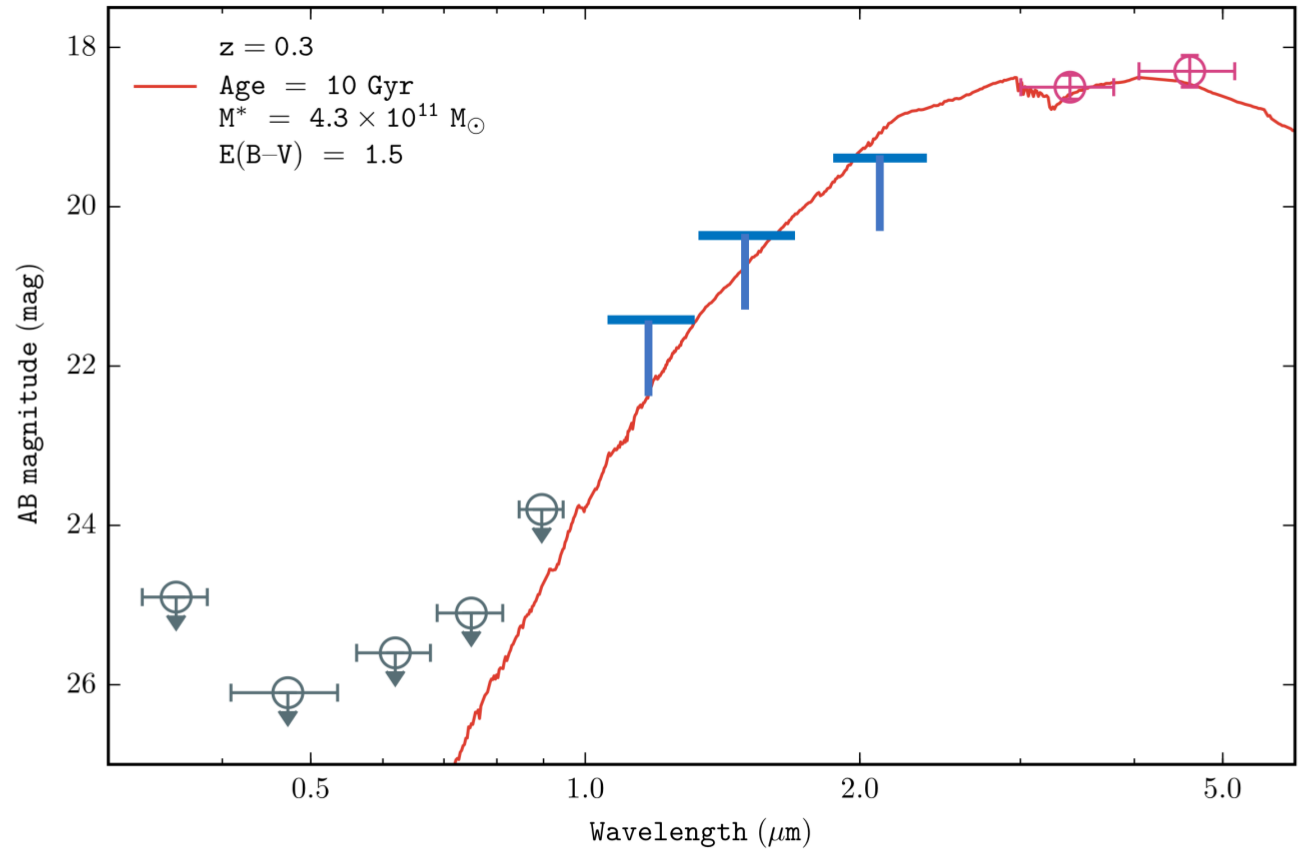
\includegraphics[width=6in]{Figures/wodrop_sed.png}
\caption{Illustration of the probable explanation to the nature of WoDrops. The photometry of this object in w1 and w2 are indicated by the two magenta points, and its non-detection in the Stripe 82 $ugriz$ images is indicated by the $2\sigma$ upper limits shown in grey.}
\label{fig:wodrop_sed}
\end{figure}

To date only quarter of the Stripe 82 footprint has been searched for the presence of WoDrops. We expect to find $\approx52,800$ dropouts. Creating the full set of WoDrops requires careful visual inspection of thousands of images, is extremely time-consuming but shall be completed in the nearest future.

We used several opportunities to add complementary photometric data to catalog. A fraction of sources is detected in IRAC SHELA - a $24 deg^{2}$ survey at 3.6 and 4.5 microns \citep{Papovich2016}. This survey is complete to 22.0 AB limiting magnitude but covers less than 10\% of Stripe 82. 

Five objects were observed with WIYN High Resolution Infrared Camera (WHIRC) \citep{Smee2011a}. Figure~\ref{fig:wodrop_whirc} shows that results are contradictory - after 3 hours of the total integration time per source only one source has detection in H and Ks, but not in J. All other sources are undetected. This non-detection is even a more interesting result as it may be a signal of detecting a new population of objects. 

\begin{figure}[!ht]
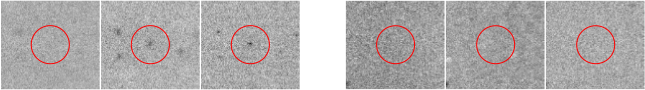
\includegraphics[width=6in]{Figures/wodrop_whirc.png}
\caption{An example of two WoDrops that have been observed by near-IR imager WHIRC instrument at WIYN telescope. All images are 33"x33" in size, and the red circles indicate the location of the WoDrop. The nominal on-source exposures are 31 min, 43 min and 1.1 hrs in Ks, but as can be seen, one WoDrop is only detected in H and Ks band, while the second one is not detected (as well as other three WoDrops that were observed in this run)}
\label{fig:wodrop_whirc}
\end{figure}

To further investigate the nature of these objects, an observing proposal was submitted to the Large Binocular Telescope (LBT) telescope to observe another 20 WoDrops (LBTO Reference: TS-2018B-006, PI - Haojing Yan). This 8m class telescope is equipped with LUCI (originally LUCIFER) - Large Binocular Telescope Near-infrared Spectroscopic Utility with Camera and Integral Field Unit for Extragalactic Research. LUCI operates in the 0.9 - 2.5 micron spectral range and provides imaging and spectroscopic capabilities in seeing- and diffraction limited modes.